\chapter{Simulador de radiología diagnóstica} 
\label{cap:xray}

En este capítulo se presenta el segundo caso de uso donde se ha integrado el algoritmo propuesto en el capítulo \ref{cap:posing}. En el simulador de radiología diagnóstica desarrollado, el objetivo es adaptar la posición del paciente virtual en tiempo real, mientras el usuario puede ver la imagen de rayos X al instante. Por tanto, en este caso la interactividad es un punto crítico, por lo cual se ha desistido de incluir la fase de optimización.

%En este capítulo, se va a mostrar otro caso de uso en esta tesis.  El algoritmo propuesto permite modificar la posición de un paciente virtual interactivamente y es posible incorporarlo en cualquier simulador que requiera una adaptación del modelo en tiempos interactivos. 
%Projectional radiography (also called projection radiography, and X-ray radiography) is a very common medical imaging tool that supports clinicians in the diagnostic of certain diseases, infections, injuries (e.g.~bone fractures), and to locate foreign objects. 
%It can be used in almost every part of the patient's body although each specific body location requires a given patient position and  X-ray machine set up, in particular collimation of the X-ray source, voltage of the X-ray tube, time of exposure, distance source to patient, and distance source to detector or film. 

La radiología diagnóstica es una técnica común que ayuda a los médicos en la diagnosis de ciertas enfermedades, infecciones y daños (p. ej. huesos fracturados). Esta técnica puede ser utilizada en cualquier parte del cuerpo del paciente pero requiere de unos conocimientos específicos. Se denomina proyecciones radiológicas al procedimiento de situar tanto al paciente como el equipo de radiología para conseguir una imagen de una parte concreta de la anatomía del paciente. Esta técnica define una proyección por cada parte del cuerpo a diagnosticar, que requiere de una postura concreta, la colimación adecuada, el voltaje de la máquina de rayos X, el tiempo de exposición y de la distancia foco-película o foco-paciente. 


En el contexto de la enseñanza de radiología diagnóstica, existen métodos de aprendizaje para ayudar al estudiante de radiología (ver sec. \ref{art:xraysim}), pero se han encontrado las siguientes limitaciones:

\begin{itemize}
\item Principalmente, los profesores usan repetidamente las mismas imágenes estáticas en sus clases, presentando el mismo caso una y otra vez.
\item No se pueden conseguir nuevas imágenes médicas instantáneamente para las clases.
\item No es posible variar la configuración de la anatomía mostrada ni conseguir diferentes anatomías para una misma configuración.
\item ProjectionVR$^{TM}$\cite{shanahan2016student} y \emph{medspace.VR} \cite{medspace} son simuladores para practicar el procedimiento en radiología diagnóstica, pero sus ejemplos son limitados.
\end{itemize}

Dadas estas limitaciones, en este capítulo se ha propuesto crear un simulador de radiología diagnóstica que pueda suplir las carencias antes citadas. Las herramientas de \ac{RV} permiten entrenar procedimientos médicos en un entorno seguro. Sobre todo, esto se vuelve especialmente importante si el entorno de trabajo no es seguro ni para pacientes ni para los propios profesionales, evitando en este caso, radiaciones peligrosas para la salud. Sin necesidad de pacientes reales, y sin límites de tiempo, estudiantes y profesores serán capaces de revisar casos diferentes, con la posibilidad de probar infinidad de configuraciones de la máquina de rayos X, e incluso enseñar como evitar errores comunes.%pudiendo trabajar con ejemplos incorrectos que no son habitualmente mostrados en la formación clásica.

%Por tanto, un simulador de \ac{RV} puede ayudar a mejorar el proceso de aprendizaje de los estudiantes de radiología. 



En colaboración con el Dr. Franck P. Vidal, se ha desarrollado un simulador de radiología diagnóstica como caso de uso del algoritmo presentado.  El usuario deberá poder cambiar la postura del paciente virtual con el objetivo de practicar las proyecciones radiológicas.
Este contará con la flexibilidad y la capacidad de %generar variabilidad anatómica
adaptar distintos modelos anatómicos del algoritmo de posicionamiento.
Así mismo, el simulador ha sido diseñado para ser flexible con el objetivo de introducir la mayor cantidad de pacientes virtuales externos. El método propuesto permitirá trabajar con modelos anatómicos incompletos y sin descripciones mecánicas, siendo necesaria únicamente la presencia de los tejidos óseos y la piel (ver sec. \ref{posing:req}). El usuario podrá modificar interactivamente la anatomía del paciente virtual con la finalidad de mover al paciente a las proyecciones radiológicas. % con una modificación de la herramienta \ac{TPTVPH}.
A su vez, la librería \emph{gVirtualXray} \cite{sujar:hal}  permitirá simular imágenes radiológicas del modelo anatómico en tiempo real. El módulo \ac{Courseware} integrará ambas tecnologías, permitiendo crear un simulador que contribuya a mejorar el entrenamiento de radiólogos noveles.


% Marcos: Tienes aclarar que este es un caso de uso de la aportación principal. En sistema necesita un algoritmo de posoing. Explica que este procedimiento implica que el radiólogo escoja la pose del paciente en tiempo real dependiendo del la proyeccion que se quiera realizar. En este escenario nuesto algoritimo de posing puede animar modelos deteallados de pacientes virtuales en tiempo real. Por otro lado solo necesita la piel y los huesos y puede animar cualquier paciente virtual. En resultados puedes comentar que modelos has incorporado, para demostrar la flexibilidad de la técnica. 

%El algoritmo será el encargado de modificar el paciente virtual  mientras que la librería \emph{gVirtualXray}\cite{sujar:hal} proporciona una imagen simulada de rayos X, todo esto  en tiempo real.
%Comentar cosas de aprendizaje por la cual necesitamos un simulador


\section{Descripción del simulador} 
\label{xray:method}

%La combinación del algoritmo propuesto en esta tesis, y la librería que permite simular rayos X permite crear un simulador para entrenar proyecciones radiológicas.
%El simulador de radiología diagnóstica permitirá a estudiantes y profesores manipular cualquier variación de anatomía humana (ver sección \ref{posing:req}) y configurar la máquina de rayos X virtual para obtener de manera inmediata una radiografía simulada. Estudiantes y profesores pueden dedicar todo el tiempo necesario en una herramienta interactiva sin riesgo ninguno frente a la práctica en un entorno real.

El simulador de radiología diagnóstica se compone de tres módulos diferenciados: el algoritmo de posicionamiento, la librería \emph{gVirtualXray} y un \ac{Courseware}. En la figura \ref{fig:Posesummary} se muestra la arquitectura del simulador.

\begin{figure}[ht]
\centering
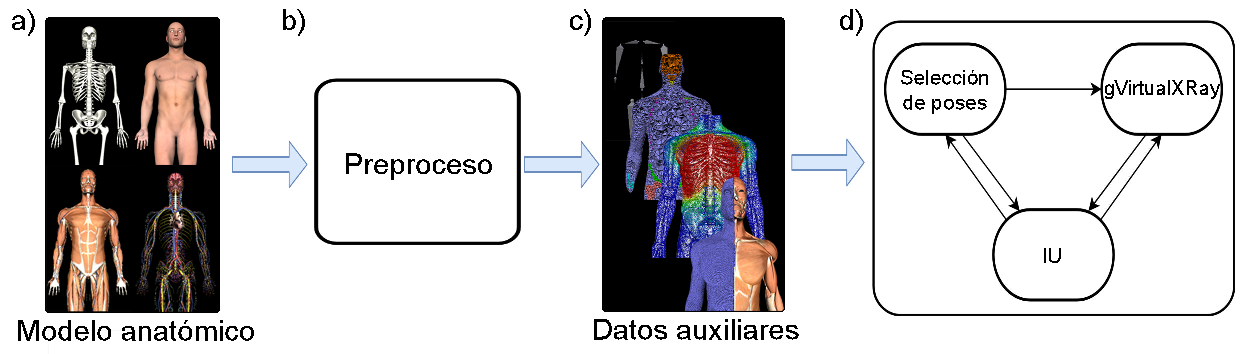
\includegraphics[width=\linewidth]{IMG/ArquXRAY.pdf}

\caption{\label{fig:Posesummary} Arquitectura del simulador: a) Modelos anatómicos de entrada; b) Proceso previo ejecutado una vez por paciente virtual; c) Datos generados necesarios para la selección de poses; d) \acs{Courseware} donde se ha integrado la \emph{selección de poses} con \emph{gVirtualXRay}.
}
\end{figure}

En primer lugar, los modelos anatómicos deberán ser preparados por el preproceso descrito en la sección \ref{posing:preprocess}. Este preproceso ejecuta las tareas más costosas computacionalmente. Este preproceso se realiza una única vez por modelo con la finalidad de generar las estructuras necesarias para el algoritmo de posicionamiento. De esta forma, el usuario podrá cargar cuantas veces quiera el modelo anatómico para adaptar la postura del paciente virtual interactivamente, gracias a la etapa de selección de poses en el simulador (ver sec. \ref{posing:Poses}). 

%Estos datos auxiliares serán cargados junto con el modelo anatómico en el simulador de radiología. 


A su vez, la librería \emph{gVirtualXray} utiliza los modelos anatómicos para mostrar la imagen de rayos X en tiempo real (ver sec. \ref{xray:setupxray}). Esta librería permite configurar los parámetros del simulador de rayos X (voltaje, distancia, etcétera), que afectará a la imagen mostrada al usuario. 

Tanto el algoritmo de posicionamiento como la librería de rayos X son computacionalmente intensas y se han integrado de forma que puedan aprovechar las capacidades de las tarjetas gráficas modernas. Debido a que ambas librerías trabajan sobre el mismo conjunto de datos, para mejorar su eficiencia, pueden compartir memoria en \acs{GPU} y, por lo tanto, conseguir una comunicación inmediata.

Por último, se ha desarrollado un módulo \ac{Courseware} que gestiona la comunicación entre los dos módulos y proporciona las funcionalidades necesarias para practicar el procedimiento. Además, puede guiar a los estudiantes a través del procedimiento fomentando el aprendizaje autónomo, o permitir resolver ejercicios propuesto por los profesores, que serán evaluados a través de los resultados y métricas almacenadas.





%El módulo \ac{Courseware} presentan en una  Por una parte, podrá observar la representación 3D de las mallas superficiales cargadas a la vez que podrá observar la imagen de rayos X en todo momento, resultado de la proyección del emisor al detector. %Esta proyección podrá ser modificada por el usuario a través del ratón o los botones diseñados para tal efecto.
%El \ac{Courseware} se ha desarrollado para integrar el algoritmo de posicionamiento y la librería \emph{gVirtualXRay}, y proporcionar una herramienta de aprendizaje donde se pueden practicar los aspectos específicos del procedimiento.


Los usuarios pueden revisar multitud de escenarios, probar parámetros de la máquina de rayos X (voltaje, colimación y distancia foco película), o focalizarse en evitar errores comunes que se realizan en los entornos reales. Además, una vez obtenida la pose del paciente virtual, el simulador permite variar la anatomía y/o los parámetros de la máquina de rayos X, frente a los archivos educativos donde solo se encuentran imágenes estáticas. El objetivo final es mejorar la confianza de los futuros profesionales médicos con vistas a reducir la dosis de radiación y el número de repeticiones en el futuro.%que sufrirán los pacientes. 


%En cuanto a la arquitectura de este simulador, citando la definición de \emph{Burdea y Coiffet} vista en la sección \ref{art:simulador}, se ha descrito los módulos que corresponden al motor de \ac{RV} y al software. En este caso, los dispositivos de \ac{E/S} son el monitor, teclado y ratón.
%Al igual que se describió en la sección permiten a la selección de poses ejecutarse interactivamente.

%La primera vez que se Se debe realizaros modelos anatómicos deben ser toma el modelo anatómico como entrada
%El \ac{Courseware} proporciona la integración y comunicación entre las dos librerías y muestra al paciente virtual a través de la interfaz de usuario.



A continuación, se va a introducir la librería \emph{gVirtualXRay} y después se pasará a describir las funcionalidades del \ac{Courseware}.


\section{gVirtualXray}
\label{xray:context}

El proyecto \emph{gVirtualXray} \cite{sujar:hal} dirigido por el Dr. Frank P. Vidal, proporciona una librería de simulación determinista de generación de imágenes radiográficas y fluoroscópicas realistas en tiempo real. %generar imágenes visualmente realistas de radiografías y fluoroscópicas.
%Una de las principales características de esta librería  es la capacidad de simular . 
La interacción es una cualidad fundamental en cualquier simulador de \ac{RV}, por lo que esta librería resulta perfecta para la creación de una aplicación de diagnóstico por imagen. 
A su vez, la librería utiliza la representación superficial de triángulos, habitualmente usada en gráficos por computador, y compatible con el algoritmo de posicionamiento.

\emph{gVirtualXray} implementa la técnica propuesta de trazador de rayos llamada \emph{L-buffer} \cite{Freud2006175}. En este método, utilizando las capacidades de la \ac{GPU}, se calcula la longitud del recorrido realizado por los rayos X que pasan a través de la malla poligonal, desde la posición del emisor de rayos X hasta cada \emph{píxel} del detector. Esto permite la posibilidad de simular eficientemente las imágenes de rayos X de cualquier objeto representado por una superficie poligonal utilizando el cauce gráfico. En la intersección rayo-polígono se resuelve la ley de \emph{Beer-Lambert} \cite{sujar:hal}, donde se relaciona la absorción de la luz (en este caso fotones) con las propiedades del material. Se utiliza la \emph{Photon Cross Sections Database (XCOM)} creada por \emph{National Institute of Standards and Technology (NIST)} \cite{XCOM} como referencia para calcular el coeficiente de atenuación másico según el material del objeto. El material puede ser descrito por su composición química o por la escala \emph{Hounsfield}.  %Esto da como resultado la posibilidad de generar imágenes visualmente realistas de radiografías y fluoroscópicas.
Para más información se puede consultar \cite{vidal2009simulation}.

Esta técnica permite la simulación en tasa de refresco interactivas, en comparación con las técnicas de  simulación de \emph{Monte Carlo}, más habituales en la bibliografía \cite{PENELOPE,badal2009}. La fidelidad de las imágenes resultantes (fig. \ref{fig:validation}), se ha validado usando \emph{Geant4} \cite{Agostinelli2003250}, una herramienta desarrollada por el \emph{European Organization for Nuclear Research (CERN)} que se encuentra como referencia en el estado del arte de la simulación de rayos X.

\begin{figure}[ht]
    \begin{subfigure}[b]{0.25\linewidth}
        \centering
        {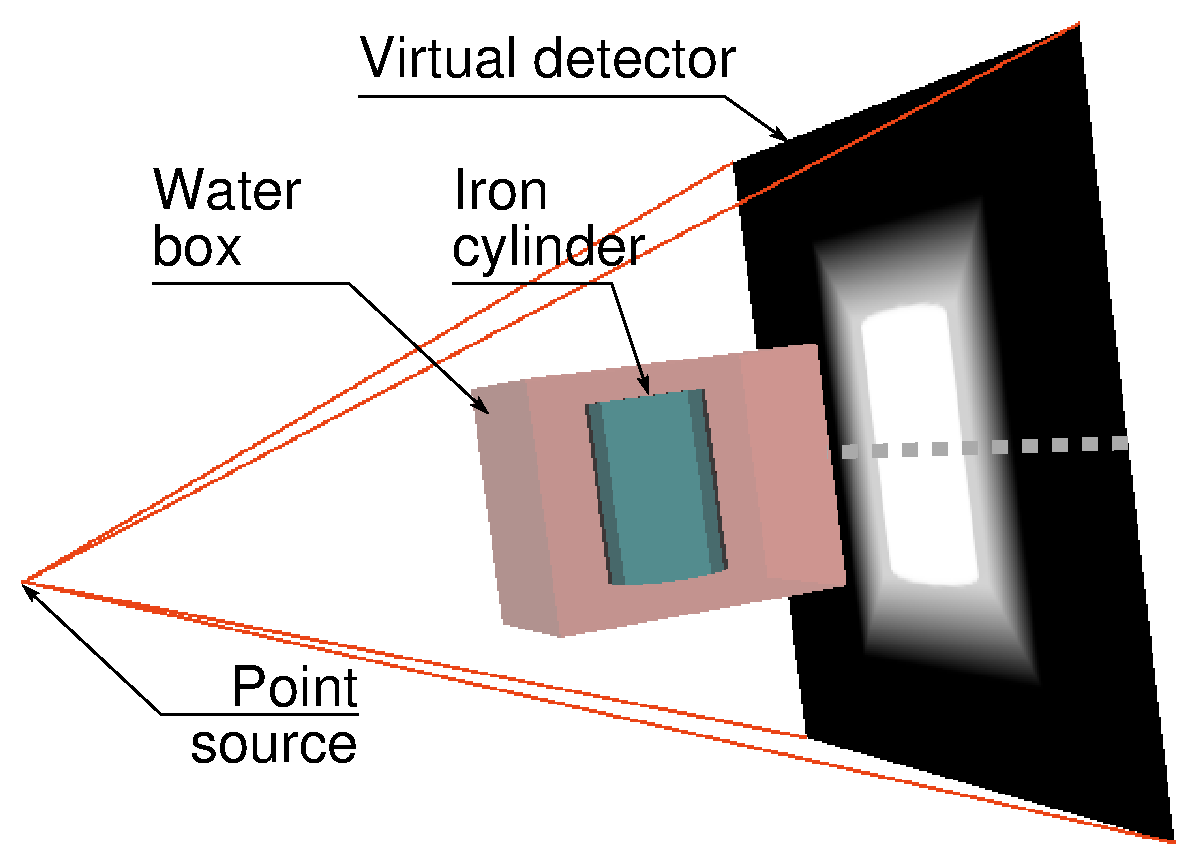
\includegraphics[width=0.8\linewidth]{IMG/figure3a.eps}}
        \caption{\label{subfig:polychromatismA} Escena de prueba.}
    \end{subfigure}
    \null\hfill
     \begin{subfigure}[b]{0.25\linewidth}
        \centering
        {\includegraphics[width=\linewidth]{IMG/figure6a.eps}}
        \caption{\label{subfig:GPU} Imagen determinista simulada  usando \emph{gVirtualXRay}.}
    \end{subfigure}
    \null\hfill
    \begin{subfigure}[b]{0.25\linewidth}
        \centering
        {\includegraphics[width=\linewidth]{IMG/figure6b.eps}}
        \caption{\label{subfig:Gate} Imagen simulada utilizando \emph{Monte Carlo} en \emph{Geant4}.}
    \end{subfigure}

\caption{\label{fig:validation} Ejemplo de la evaluación para la herramienta \emph{gVirtualXRay} \cite{sujar:hal}.}
\end{figure}











